\documentclass{article}
\usepackage[italian]{babel}
\usepackage{graphicx} % Required for inserting images
\graphicspath{{./figures/}}
\usepackage{hyperref}
\usepackage{float}
\usepackage{amsmath}

\title{\textbf{Relazione Progetto Gpu Computing \\ \Large Ray Tracing}}
\author{Andrea Longoni\\(13896A)}
\date{}

\begin{document}

\maketitle

% \tableofcontents

\section{Introduzione}

L'obiettivo di questo progetto è di implementare un ray tracer, un programma capace di generare immagini che rappresentano una scena tridimensionale.
Un raytracer è un programma che simula il comportamento della luce per determinare il colore di ogni pixel di un'immagine, tracciando il percorso dei raggi di luce che interagiscono con gli oggetti in una scena 3D.
Poiché il calcolo del colore di ciascun pixel può essere eseguito indipendentemente dagli altri, l'algoritmo è particolarmente adatto per essere parallelizzato, sfruttando la potenza di calcolo delle GPU.

Nel progetto, ho implementato due versioni dell'algoritmo di ray tracing: una versione sequenziale eseguita esclusivamente su CPU, e una versione parallela ottimizzata per l'esecuzione su GPU.
Il programma sviluppato permette di creare file in formato \texttt{PPM}, \texttt{BMP} o \texttt{GIF} animate, nei quali vengono rappresentati vari oggetti 3D, come sfere, piani e modelli 3D in formato \texttt{.obj}.
Questi oggetti possono avere texture di vari tipi: monocromatiche, a scacchiera o basate su immagini, con supporto per texture definite nei file \texttt{.obj} e \texttt{.mtl}.

In questa relazione, descriverò brevemente il funzionamento dell'algoritmo e i dettagli implementativi delle due versioni. Successivamente, analizzerò i risultati ottenuti confrontando i tempi di esecuzione su CPU e GPU, evidenziando i miglioramenti di performance ottenuti grazie al parallelismo.\\

Il codice sorgente e ulteriori dettagli sull'implementazione del progetto sono disponibili nel repository GitHub, accessibile tramite il seguente link:\\\centerline{\url{https://github.com/Andreal2000/Project-Ray-Tracing}}.

\section{Descrizione dell'Algoritmo}

Per ogni pixel dell'immagine, l'algoritmo traccia un raggio dalla posizione della camera (che rappresenta l'osservatore virtuale) verso un punto specifico di un rettangolo chiamato viewport, che rappresenta la proiezione della scena 3D sul piano 2D dell'immagine.

La direzione del raggio viene calcolata come la differenza tra la posizione della camera e il punto corrispondente nel viewport.
Una volta tracciato il raggio, l'algoritmo determina se esso interseca uno degli oggetti presenti nella scena e, in tal caso, individua l'oggetto più vicino e il punto esatto di collisione.\\

Il colore del pixel corrispondente viene quindi determinato utilizzando il modello di illuminazione di Phong\cite{Phong}, che combina tre componenti principali:

\begin{itemize}
    \item \textbf{Componente Ambientale:} Questa componente rappresenta la luce diffusa presente in tutta la scena, indipendentemente dalla posizione e direzione delle sorgenti luminose. Contribuisce a evitare che le aree non direttamente illuminate siano completamente nere. La componente ambientale è espressa come:

    \[ I_a = k_a \cdot I_{a, \text{globale}} \]

    Dove \(I_a\) è l'intensità della componente ambientale, \(k_a\) è il coefficiente di riflessione ambientale del materiale, e \(I_{a, \text{globale}}\) è l'intensità della luce ambientale globale.
    
    \item \textbf{Componente Diffusa:} Determinata dall'orientamento della superficie rispetto alla sorgente luminosa. Viene calcolata considerando l'angolo tra la normale alla superficie nel punto di impatto (\(\vec{N}\)) e la direzione della luce (\(\vec{L}\)). Maggiore è la perpendicolarità tra la luce e la superficie, più intensa sarà questa componente, che dà l'idea di come la luce colpisce direttamente l'oggetto. Poiché questa componente dipende dalla posizione della luce, deve essere calcolata per ogni sorgente luminosa presente nella scena. La componente diffusa totale è quindi data dalla somma dei contributi di tutte le luci:

    \[ I_d = \sum_{\text{luci}} \left( k_d \cdot I_l \cdot \max(\vec{N} \cdot \vec{L}, 0) \right) \]

    Dove \(I_d\) è l'intensità complessiva della componente diffusa, \(k_d\) è il coefficiente di riflessione diffusa del materiale, \(I_l\) è l'intensità della luce proveniente da una singola sorgente, e \(\max(\vec{N} \cdot \vec{L}, 0)\) assicura che il contributo sia non negativo.

    \item \textbf{Componente Speculare:} Rappresenta il riflesso della luce sulla superficie, creando un effetto di lucentezza. Viene calcolata in base alla direzione della luce riflessa (\(\vec{R}\)) rispetto alla direzione dell'osservatore (\(\vec{V}\)), simulando il riflesso della luce su materiali lucidi o metallici. Come per la componente diffusa, anche la componente speculare deve essere calcolata per ogni sorgente luminosa, poiché dipende dalla posizione della luce riflessa (\(\vec{R}\)) rispetto alla direzione dell'osservatore (\(\vec{V}\)). La componente speculare totale è data da:

    \[ I_s = \sum_{\text{luci}} \left( k_s \cdot I_l \cdot \max(\vec{R} \cdot \vec{V}, 0)^n \right) \]

    Dove \(I_s\) è l'intensità complessiva della componente speculare, \(k_s\) è il coefficiente di riflessione speculare del materiale, \(I_l\) è l'intensità della luce proveniente da una singola sorgente, \(\vec{R}\) è la direzione del riflesso della luce, \(\vec{V}\) è la direzione dell'osservatore, e \(n\) è un esponente che determina la lucentezza (più è grande, più il riflesso è concentrato).
\end{itemize}

Il colore finale del pixel viene quindi calcolato sommando la componente ambientale unica e le componenti diffuse e speculari, che tengono conto di tutte le luci nella scena:

\[ I = I_a + I_d + I_s \]

Se il raggio colpisce più oggetti, viene considerato solo l'oggetto più vicino alla camera. Inoltre, per simulare effetti realistici come le ombre, viene tracciato un ulteriore raggio verso ciascuna sorgente luminosa per verificare se essa è visibile dal punto di collisione o se è oscurata da altri oggetti.

\section{Descrizione dell'Implementazione}

\subsection{Modello CUDA per il Ray Tracing}

Il ray tracing è un algoritmo che si presta naturalmente al parallelismo, poiché ogni pixel dell'immagine può essere calcolato in modo indipendente dagli altri. Questa caratteristica lo rende particolarmente adatto per essere implementato utilizzando il modello di programmazione CUDA, che consente di sfruttare la potenza di calcolo delle GPU.

Nella mia implementazione, ho scelto di assegnare un thread CUDA a ciascun pixel dell'immagine. Ogni thread è responsabile del calcolo del colore del pixel corrispondente, tracciando il raggio attraverso la scena e applicando il modello di illuminazione di Phong. Per ottimizzare l'uso delle risorse della GPU e ridurre la divergenza tra i thread, ho suddiviso i thread in blocchi, con ciascun blocco che gestisce una sezione di pixel 8x8.

Questa suddivisione è stata scelta per sfruttare al meglio la coerenza spaziale dei raggi vicini. Raggi che attraversano pixel adiacenti tendono a interagire con gli stessi oggetti nella scena e a seguire percorsi simili. Di conseguenza, i thread all'interno dello stesso blocco avranno maggiori probabilità di eseguire istruzioni simili, riducendo la divergenza dei thread all'interno del blocco. La riduzione della divergenza è cruciale per mantenere l'efficienza della GPU, poiché quando i thread all'interno di un warp (gruppo di thread eseguiti simultaneamente) seguono percorsi di esecuzione diversi, la GPU deve serializzare l'esecuzione, causando un rallentamento.

In aggiunta al calcolo del colore basato sul modello di illuminazione di Phong, ogni thread gestisce anche l'oversampling del pixel. Questa tecnica di antialiasing migliora la qualità dell'immagine finale, il colore di ciascun pixel viene calcolato più volte, variando leggermente la direzione del raggio all'interno del pixel. Il thread calcola quindi la media dei colori ottenuti per determinare il colore finale del pixel.

\subsection{Utilizzo della Libreria cuRAND per l'Antialiasing}

Per implementare l'antialiasing nel ray tracing, è essenziale generare numeri casuali che permettano di variare leggermente la direzione del raggio all'interno di ciascun pixel. Questo processo, noto come oversampling, richiede un campionamento casuale all'interno del pixel per calcolare il colore più volte e ottenere una media che rappresenti il colore finale. L'obiettivo è ridurre l'effetto di aliasing, ovvero la scalettatura dei bordi nell'immagine.

Per introdurre queste variazioni casuali nelle direzioni dei raggi, è essenziale disporre di numeri casuali di alta qualità. A questo scopo, ho utilizzato la libreria cuRAND, una libreria fornita da NVIDIA che consente di generare numeri casuali direttamente sulla GPU in modo altamente efficiente.

L'utilizzo di cuRAND è particolarmente vantaggioso in un contesto di calcolo parallelo come quello offerto dal modello CUDA. Ogni thread, responsabile del calcolo di un pixel, può generare i propri numeri casuali per determinare le variazioni nelle direzioni dei raggi.

Per ogni pixel, i numeri casuali generati da cuRAND vengono utilizzati per perturbare leggermente la direzione del raggio, creando una serie di raggi che attraversano diverse posizioni nelle prossimità del pixel. Il colore finale del pixel viene quindi determinato dalla media dei colori ottenuti da questi raggi, garantendo un'immagine più morbida e priva di artefatti di aliasing.

\subsection{Gestione della Memoria}
La gestione della memoria è un aspetto cruciale nell'implementazione di un qualunque programma che lavori con la GPU, specialmente quando si tratta di oggetti complessi come quelli presenti in una scena tridimensionale. Nel mio progetto, la scena 3D è rappresentata da una gerarchia di oggetti che estendono una classe astratta chiamata \texttt{Hittable}. Questa struttura permette di modellare vari elementi della scena, come sfere, piani e modelli 3D, ciascuno con comportamenti specifici in termini di interazione con i raggi tracciati.

Il principale problema incontrato durante lo sviluppo riguarda la corretta gestione della memoria per gli oggetti della scena, dovuta al fatto che la GPU ha il suo spazio di memoria separato dalla CPU. Quando un oggetto che estende una classe astratta come \texttt{Hittable} o \texttt{Texture} viene istanziato, è necessario assicurarsi che la sua Virtual Method Table (VMT) sia correttamente allocata nella memoria della GPU. Questo è essenziale perché, se l'oggetto fosse allocato in memoria sulla CPU e poi copiato sulla GPU, la VMT punterebbe a indirizzi di memoria non validi sulla GPU, causando errori di accesso alla memoria.\\

Per risolvere questo problema, ho adottato la seguente strategia:

\begin{enumerate}
    \item \textbf{Allocazione della Memoria:} Utilizzo \texttt{cudaMalloc} per allocare la memoria necessaria per gli oggetti su GPU. Questa memoria viene poi passata a un kernel CUDA che si occupa di costruire gli oggetti direttamente nell'area di memoria della GPU. Questo assicura che la VMT degli oggetti risieda nella memoria GPU, permettendo ai kernel di accedere correttamente ai metodi virtuali.
    
    \item \textbf{Deallocazione della Memoria:} Una volta che gli oggetti non sono più necessari, devono essere deallocati correttamente. Poiché la deallocazione deve avvenire sulla GPU, ho scritto un kernel CUDA specifico che prende in input i puntatori agli oggetti e ne esegue la deallocazione tramite \texttt{delete}. Successivamente, la memoria allocata con \texttt{cudaMalloc} viene liberata usando \texttt{cudaFree}.
\end{enumerate}

Alcuni oggetti, come la \texttt{Camera}, richiedono di operare sia sulla CPU che sulla GPU. Per gestire questi casi, ho utilizzato la memoria unificata offerta da CUDA tramite \texttt{cudaMallocManaged}. Questa tecnica permette di allocare oggetti in un'area di memoria accessibile sia dalla CPU che dalla GPU, facilitando la condivisione dei dati tra i due processori. Per semplificare l'allocazione e la deallocazione di questi oggetti, ho fatto in modo che estendessero una classe chiamata \texttt{Managed}, che ridefinisce gli operatori \texttt{new} e \texttt{delete} per utilizzare \texttt{cudaMallocManaged} e \texttt{cudaFree}, rispettivamente. Cosi facendo è possibile rendere trasparente la gestione della memoria per gli oggetti condivisi, riducendo il rischio di errori e semplificando il codice.

Questo approccio alla gestione della memoria assicura che tutte le risorse siano gestite correttamente, evitando fughe di memoria e garantendo che i kernel CUDA possano accedere e manipolare gli oggetti della scena senza incorrere in errori di accesso alla memoria. Per confermare l'assenza di memory leak, il codice è stato testato utilizzando il tool \texttt{NVIDIA Compute Sanitizer}\cite{NVIDIA-Compute-Sanitizer}, che ha verificato l'integrità della gestione della memoria nel programma.

\subsection{File di Output}

Una volta terminato il processo di calcolo di tutti i pixel del immagine il programma è in grado di generare tre tipi di file di output: \texttt{PPM} (Netpbm)\cite{PPM}, \texttt{BMP} (Bitmap)\cite{BMP} e \texttt{GIF} (GIF89a)\cite{GIF}. Ciascuno di questi formati rappresenta l'immagine in modo diverso, e solo una parte del processo di generazione delle \texttt{GIF} è stato accelerato utilizzando la GPU.

\subsubsection{Formato PPM (Netpbm)}

Il formato \texttt{PPM} è tra i più semplici in termini di struttura. I dati di un'immagine \texttt{PPM} sono codificati come una sequenza di valori RGB, dove ogni pixel è rappresentato da tre numeri che indicano l'intensità del rosso, verde e blu. Questi valori sono organizzati in un formato che può essere sia testuale (dove i numeri sono scritti in ASCII) sia binario (dove i numeri sono scritti in byte). Il file inizia con un'intestazione che include informazioni come la larghezza e l'altezza dell'immagine e il valore massimo per i colori, seguita dai dati pixel per pixel.
Il programma prima calcola i colori di tutti i pixel dell'immagine usando la GPU e successivamente scrive questi valori su file in modo sequenziale.

\subsubsection{Formato BMP (Bitmap)}

Il formato \texttt{BMP} ha una struttura più complessa, ma rimane relativamente semplice. Il file inizia con un'intestazione che descrive le dimensioni dell'immagine, il numero di bit per pixel, e altre informazioni sulla struttura del file. Successivamente, i dati dei pixel sono organizzati in una matrice che rappresenta l’immagine, con i valori di colore memorizzati in ordine inverso (BGR anziché RGB). Poiché il formato BMP non comprime i dati, ogni pixel occupa uno spazio fisso, il che rende il formato semplice ma inefficiente in termini di spazio. Analogamente al file \texttt{PPM}, anche il file \texttt{BMP} è generato interamente dalla CPU dopo che i colori dei pixel sono stati calcolati sulla GPU.

\subsubsection{Formato GIF (GIF89a)}

Il formato \texttt{GIF} è più complesso rispetto ai precedenti, poiché supporta l'animazione e la compressione. Una \texttt{GIF} è composta da una serie di fotogrammi (frame), dove ogni frame rappresenta un’immagine della scena, ciascuno rappresentato da una lista di pixel. Ogni pixel viene associato a un colore presente in una palette, generalmente composta da un massimo di 256 colori.

Il programma non genera una singola immagine statica, ma applica una rotazione della camera attorno alla scena per ogni frame. Alla fine della sequenza, la camera ritorna al punto di partenza, creando un effetto di loop continuo senza interruzioni o scatti.\\

Il processo di generazione della \texttt{GIF} è suddiviso in diverse fasi:
\begin{itemize}
    \item \textbf{Quantizzazione dei Colori:} Prima di tutto, il programma esegue una quantizzazione dei colori per ridurre il numero di colori dell'immagine a quelli presenti nella palette. Questo processo è eseguito sulla CPU.

    \item \textbf{Mapping dei Colori:} Una volta creata la palette, ogni pixel deve essere mappato al colore più simile presente nella palette. Questa operazione è stata accelerata con l'uso della GPU, sfruttando il parallelismo per trovare rapidamente il colore più simile per ogni pixel. Questo passaggio migliora notevolmente le prestazioni rispetto a una soluzione puramente CPU-based.

    \item \textbf{Compressione (LZW):} Dopo il mapping dei colori, ogni frame della \texttt{GIF} viene compresso utilizzando l'algoritmo LZW (Lempel-Ziv-Welch)\cite{LZW}, che è parte integrante del formato \texttt{GIF}. Questo processo riduce le dimensioni del file finale e viene eseguito sulla CPU.
\end{itemize}

\subsection{Ottimizzazione con Bounding Box}

Uno degli aspetti più onerosi in termini di calcolo è determinare con precisione quale oggetto nella scena è stato colpito da un raggio. Questo problema diventa particolarmente rilevante quando si lavora con modelli 3D complessi composti da migliaia di triangoli. Per ottimizzare questa operazione e migliorare le prestazioni del raytracer, è stata implementata un’ottimizzazione che utilizza le bounding box.

Una bounding box è un semplice parallelepipedo che racchiude interamente un oggetto 3D. In pratica, invece di testare immediatamente se un raggio ha colpito i singoli triangoli di un modello 3D, si verifica prima se il raggio interseca la bounding box dell'oggetto. Se il raggio non colpisce la bounding box, è inutile controllare i singoli poligoni all'interno di essa, poiché l'oggetto non può essere stato colpito. Questo riduce drasticamente il numero di controlli necessari, specialmente in scene con geometrie complesse.\\

L’ottimizzazione con bounding box offre un doppio vantaggio:
\begin{itemize}
    \item \textbf{Efficienza nei calcoli:} Nei casi in cui un raggio non colpisce alcun oggetto, l'algoritmo può terminare rapidamente, calcolando solo l'intersezione con le bounding box e non con i poligoni dettagliati all'interno. Ciò è particolarmente utile in scene sparse, dove molti raggi non colpiscono alcun oggetto.

    \item \textbf{Riduzione dei test geometrici:} Per i raggi che effettivamente colpiscono un oggetto, la bounding box permette di evitare molti test inutili sui singoli triangoli, migliorando le prestazioni complessive. Questo è particolarmente evidente nei modelli con molti poligoni, dove la probabilità di colpire effettivamente un poligono specifico è bassa senza questa ottimizzazione.
\end{itemize}

\section{Confronto delle Performance}

In questa sezione, discuteremo le performance del raytracer confrontando l'esecuzione su CPU e GPU in vari scenari.\\

Tutti i test sono stati eseguiti su una macchina dotata delle seguenti caratteristiche hardware:

\begin{itemize}
    \item \textbf{Processore (CPU):} AMD Ryzen 5 3600 @ 3.60GHz
    \item \textbf{Scheda Grafica (GPU):} NVIDIA GeForce RTX 1660 SUPER
    \item \textbf{Memoria (RAM):} 16 GB DDR4
\end{itemize}

Sono state testate cinque diverse scene, variando le condizioni di esecuzione per includere o escludere il antialiasing (AA) e l'uso delle bounding box (BB). In alcuni casi, è stata generata anche una \texttt{GIF} animata.

Tutte le immagini sono state generate in formato Bitmap e hanno una risoluzione di 500x500 pixel, quando l'antialiasing è abilitato, il numero di campioni per pixel è stato impostato a 64. Per le \texttt{GIF} animate, la durata è stata fissata a 5 secondi con una frequenza di 24 fotogrammi al secondo (fps).
    
\subsection{Balls}

\begin{figure}[H]
    \centering
    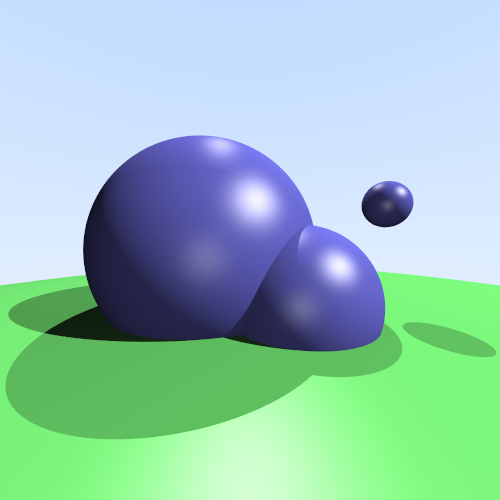
\includegraphics[width=0.5\linewidth]{balls.png}
    % \caption{Enter Caption}
    \label{fig:balls}
\end{figure}

Nel primo test, è stata utilizzata una scena relativamente semplice composta da:
Quattro sfere con texture monocromatiche e tre luci ma senza luce ambientale.\\

I risultati dei test sono i seguenti:

\begin{table}[H]
    \centering
    \begin{tabular}{|l|r|r|}
    \hline
    \textbf{Modificatori} & \textbf{CPU (ms)}   & \textbf{GPU (ms)} \\ \hline
    Nessuno      & 256   & 11  \\ \hline
    AA           & 16954 & 654 \\ \hline
    BB           & 327   & 12  \\ \hline
    AA + BB      & 20868 & 704 \\ \hline
    \end{tabular}
\end{table}

Per questa scena è stata generata anche una \texttt{GIF} e i tempi di esecuzione sono i seguenti:

\begin{table}[H]
    \centering
    \begin{tabular}{|l|r|r|}
    \hline
    \textbf{Operazione} & \textbf{CPU (ms)} & \textbf{GPU (ms)} \\ \hline
    Rendering  & 30806  & 1190  \\ \hline
    Exporting  & 205969 & 58154 \\ \hline
    \end{tabular}
\end{table}

\subsection{Earth}

\begin{figure}[H]
    \centering
    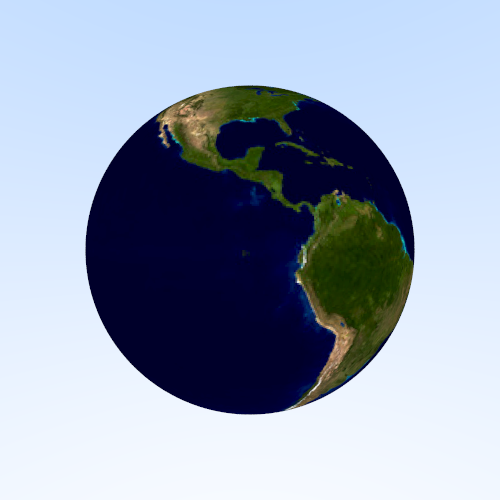
\includegraphics[width=0.5\linewidth]{earth.png}
    % \caption{Enter Caption}
    \label{fig:earth}
\end{figure}

Nel secondo test, si mostrano le capacità di rendering di una sfera su cui è stata applicata una texture presa da un immagine.\\

I risultati dei test sono i seguenti:

\begin{table}[H]
    \centering
    \begin{tabular}{|l|r|r|}
    \hline
    \textbf{Modificatori} & \textbf{CPU (ms)}   & \textbf{GPU (ms)} \\ \hline
    Nessuno      & 63   & 3   \\ \hline
    AA           & 4792 & 178 \\ \hline
    BB           & 74   & 3   \\ \hline
    AA + BB      & 5478 & 201 \\ \hline
    \end{tabular}
\end{table}

Per questa scena è stata generata anche una \texttt{GIF} e i tempi di esecuzione sono i seguenti:

\begin{table}[H]
    \centering
    \begin{tabular}{|l|r|r|}
    \hline
    \textbf{Operazione} & \textbf{CPU (ms)} & \textbf{GPU (ms)} \\ \hline
    Rendering  & 7542   & 334   \\ \hline
    Exporting  & 202002 & 52819 \\ \hline
    \end{tabular}
\end{table}

\subsection{Cornell Box}

\begin{figure}[H]
    \centering
    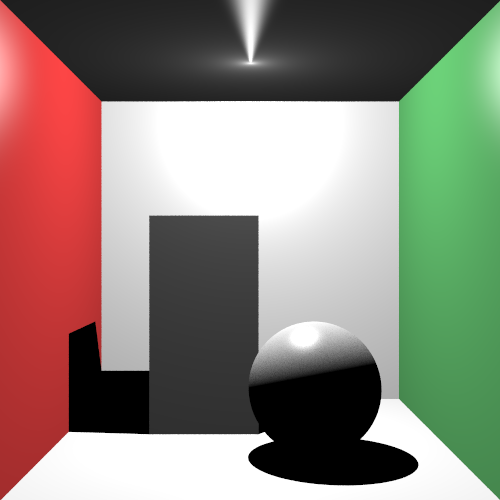
\includegraphics[width=0.5\linewidth]{cornell_box.png}
    % \caption{Enter Caption}
    \label{fig:cornell_box}
\end{figure}

Il test sulla Cornell Box\cite{Cornell} è stato progettato per valutare le prestazioni del raytracer su una scena di riferimento classica nel campo del rendering, nota per la sua semplicità e utilità nella verifica dell'accuratezza dell'illuminazione e delle ombre.

La Cornell Box è una scena composta da una semplice scatola con pareti di colori distintivi e all'interno una sfera e un parallelepipedo.\\

I risultati dei test sono i seguenti:

\begin{table}[H]
    \centering
    \begin{tabular}{|l|r|r|}
    \hline
    \textbf{Modificatori} & \textbf{CPU (ms)}   & \textbf{GPU (ms)} \\ \hline
    Nessuno      & 349   & 15  \\ \hline
    AA           & 23069 & 858 \\ \hline
    BB           & 360   & 13  \\ \hline
    AA + BB      & 24033 & 748 \\ \hline
    \end{tabular}
\end{table}

Per questa scena non è stata generata una \texttt{GIF} poiché la rotazione attorno alla scatola avrebbe prodotto molti frame completamente neri, dato che non ci sono luci all'esterno della scatola.

\subsection{Stanford Bunny}

\begin{figure}[H]
    \centering
    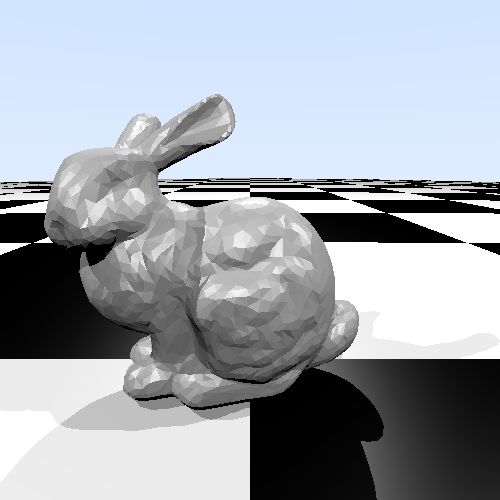
\includegraphics[width=0.5\linewidth]{bunny.png}
    % \caption{Enter Caption}
    \label{fig:bunny}
\end{figure}

Nel test con lo Stanford Bunny\cite{Bunny}, l'obiettivo era valutare le prestazioni del ray tracer con un modello complesso composto da un elevato numero di poligoni, nello specifico 4968 triangoli. Questo modello 3D presenta una geometria dettagliata che richiede un numero significativo di calcoli per determinare le intersezioni tra i raggi e le superfici, in aggiunta sono state posizionate quattro luci che aumentano la complessità del operazione.\\

I risultati dei test sono i seguenti:

\begin{table}[H]
    \centering
    \begin{tabular}{|l|r|r|}
    \hline
    \textbf{Modificatori} & \textbf{CPU (ms)}   & \textbf{GPU (ms)} \\ \hline
    Nessuno      & 239486 & 10096 \\ \hline
    % AA           &        &       \\ \hline
    BB           & 127027 & 5664  \\ \hline
    % AA + BB      &        &       \\ \hline
    \end{tabular}
\end{table}

Per questa scena, i test con l'antialiasing non sono stati eseguiti a causa dell'elevato tempo di calcolo necessario anche senza l'antialiasing. Considerando che l'antialiasing richiede 64 campioni per pixel, si può stimare un tempo di rendering circa 64 volte superiore rispetto al tempo impiegato senza antialiasing. Allo stesso modo, non è stata generata una \texttt{GIF}, poiché il calcolo avrebbe richiesto un tempo significativamente maggiore.

\subsection{Spot}

\begin{figure}[H]
    \centering
    
\includegraphics[width=0.5\linewidth]{spot.png}
    % \caption{Enter Caption}
    \label{fig:spot}
\end{figure}

Nel test con l'asset Spot\cite{Spot} è stato valutato il rendering di un modello 3D complesso (5856 triangoli), che utilizza mappatura UV per applicare una texture dettagliata. Il file \texttt{.obj} dell'asset definisce i punti di mappatura sulla superficie del modello, permettendo di visualizzare la texture correttamente applicata sui punti specificati.\\

I risultati dei test sono i seguenti:

\begin{table}[H]
    \centering
    \begin{tabular}{|l|r|r|}
    \hline
    \textbf{Modificatori} & \textbf{CPU (ms)}   & \textbf{GPU (ms)} \\ \hline
    Nessuno      & 69943 & 3459   \\ \hline
    AA           &       & 121075 \\ \hline
    BB           & 49463 & 2323   \\ \hline
    AA + BB      &       & 80591  \\ \hline
    \end{tabular}
\end{table}

Come per la scena precedente alcuni test non sono stati eseguiti a causa dell'elevato tempo di calcolo.


\subsection{Analisi dei Risultati}

L'analisi dei risultati dei test condotti evidenzia i vantaggi e le sfide dell'utilizzo della GPU rispetto alla CPU. In generale, l'adozione della GPU ha portato a una significativa riduzione dei tempi di rendering e di creazione delle \texttt{GIF}, con miglioramenti notevoli nelle prestazioni.

\textbf{Rendering Generale:} L'uso della GPU ha comportato una riduzione media dei tempi di rendering di circa 25 volte rispetto alla CPU.

\textbf{Antialiasing:} Come prevedibile il tempo di rendering è aumentato in modo significativo con l'antialiasing attivato, a causa del elevato di campioni necessari per ogni pixel.

\textbf{Bounding Box:} L'implementazione delle bounding box ha migliorato notevolmente le prestazioni nelle scene dove è presente un modello 3D, mentre per oggetti semplici come sfere o piani si è avuto un rallentamento. Questo avviene perché l'algoritmo deve comunque eseguire il controllo di intersezione con la bounding box e, se positivo, procedere con l'intersezione dell'oggetto stesso. Questo doppio passaggio può risultare inefficiente quando l'intersezione con l'oggetto è già rapida da calcolare.

\textbf{GIF Animata:} L'esportazione della \texttt{GIF} animata ha mostrato un miglioramento medio di circa 3 volte con la GPU, semplicemente con l'aggiunta del kernel per la mappatura dei colori dei pixel con la palette della \texttt{GIF}.

\section{Conclusioni}

Il progetto di ray tracing ha dimostrato chiaramente i benefici del parallelismo offerto dall'architettura CUDA rispetto all'esecuzione sequenziale su CPU. Le misurazioni delle performance mostrano miglioramenti significativi nei tempi di rendering e di esportazione delle immagini. In particolare, l'uso delle GPU ha permesso una riduzione media di 25 volte nei tempi di rendering e di 3 volte per l'esportazione delle \texttt{GIF}.

\bibliographystyle{unsrt}
\bibliography{biblio}

\end{document}
